\scanpage{23}
Soit maintenant $\beta\in I\setminus K$, prouvons que l'on a $\overline V\cap E_\beta=\varnothing$. En effet, $V$ ne \deleted{contient} \inserted{rencontre} aucun $E_i$ $(i\in I)$ donc
% BEGIN GROUP C023-G01
% Full-scan origin (98,437); local rectangle (0,0)--(9,10); baseline (0,0).
% Owns only the left detached trace M01; no adjacent word or E_beta is included.
\reversemarginpar\margin{\unsure{\begin{tikzpicture}[x=.22pt,y=-.22pt,baseline={(0,0)}]
\path[use as bounding box] (0,0) rectangle (9,10);
% path C023-G01-P01: dark triangular head and fading short lower tail.
\fill[black!70] (3,3) -- (6,2) -- (6,5) -- (4,8) -- cycle;
\end{tikzpicture}}}\normalmarginpar
% END GROUP C023-G01
$E_\beta\subset X\setminus V=
% BEGIN GROUP C023-G02
% Full-scan origin (710,414); rectangle (-20,0)--(90,122); baseline (0,62).
% Whole-state candidates: deleted bigvee followed by live bigcup | retraced live bigcup.
% Owns the first operator and its complete alpha-in-K lower label, once.
\mathop{\unsure{\text{\begin{tikzpicture}[x=.20pt,y=-.20pt,baseline={(0,62)}]
\path[use as bounding box] (-20,0) rectangle (90,122);
\node[overlay,anchor=base west,inner sep=0,outer sep=0] at (0,0) {\phantom{$\deleted{\bigvee}\bigcup\mid\bigcup$}};
% path C023-G02-P01: outer cup, including both stalks and the lower return.
\draw[line width=.65pt,line cap=round] (13,8) .. controls (14,27) and (12,49) .. (20,55) .. controls (29,64) and (38,55) .. (43,42) .. controls (48,29) and (49,15) .. (50,5);
% path C023-G02-P02: oblique inner run with its short upturned lower end.
\draw[line width=.48pt,line cap=round] (7,15) .. controls (18,29) and (21,41) .. (27,50) .. controls (32,56) and (36,50) .. (39,45);
% label C023-G02-L01: alpha in K, complete and not repeated outside this group.
\node[anchor=base west,inner sep=0,outer sep=0] at (-18,112) {$\scriptstyle\alpha\in K$};
\end{tikzpicture}}}}
% END GROUP C023-G02
% BEGIN GROUP C023-G03
% Full-scan origin (807,386); rectangle (0,0)--(95,95); baseline (0,72).
% Whole-state candidates: widehat{deleted I Sigma}_alpha^+ | widehat{deleted E Sigma}_alpha^+ | widehat{Sigma}_alpha^+ with internal retrace.
% Owns S01: roof, joined head/body, internal upright, plus and alpha; no operator or comma.
\unsure{\text{\begin{tikzpicture}[x=.20pt,y=-.20pt,baseline={(0,72)}]
\path[use as bounding box] (0,0) rectangle (95,95);
\node[overlay,anchor=base west,inner sep=0,outer sep=0] at (0,0) {\phantom{$\widehat{\deleted{I}\Sigma}_\alpha^+\mid\widehat{\deleted{E}\Sigma}_\alpha^+\mid\widehat\Sigma_\alpha^+$}};
% path C023-G03-P01: Sigma head and angular body, joined at their left start.
\draw[line width=.66pt,line cap=round] (7,31) .. controls (19,27) and (33,29) .. (49,30) (13,32) .. controls (24,38) and (36,41) .. (40,49) .. controls (40,55) and (24,64) .. (14,71) -- (55,70);
% path C023-G03-P02: internal upright, whose predecessor/retrace role remains unresolved.
\draw[line width=.64pt,line cap=round] (29,39) .. controls (31,47) and (30,60) .. (32,70);
% path C023-G03-P03: separate roof above the corrected glyph.
\draw[line width=.65pt,line cap=round] (41,18) .. controls (51,16) and (58,10) .. (64,5) .. controls (72,12) and (79,17) .. (84,18);
% path C023-G03-P04: raised plus, both components.
\draw[line width=.65pt,line cap=round] (65,42) -- (82,40) (72,35) -- (75,49);
% label C023-G03-L01: lower alpha.
\node[anchor=base west,inner sep=0,outer sep=0] at (63,84) {$\scriptstyle\alpha$};
\end{tikzpicture}}}
% END GROUP C023-G03
$, \deleted{\unsure{donc si}} je dis que si $\beta\in I\setminus K$,
% BEGIN GROUP C023-G04
% Full-scan origin (943,550); rectangle (0,0)--(190,80); baseline (0,65).
% Owns exactly the live words on a and ochre trace M02; en fait remains outside.
\begin{tikzpicture}[x=.18pt,y=-.18pt,baseline={(0,65)}]
\path[use as bounding box] (0,0) rectangle (190,80);
\node[anchor=base west,inner sep=0,outer sep=0] at (0,65) {on a};
% The nested trace has origin (1115,560), baseline (0,0), and zero-separation base-west anchor.
\node[anchor=base west,inner sep=0,outer sep=0] at (172,10) {\unsure{\begin{tikzpicture}[x=.18pt,y=-.18pt,baseline={(0,0)}]
\path[use as bounding box] (0,0) rectangle (10,10);
% path C023-G04-P01: isolated ochre oblique shape; role, hand and surface origin undetermined.
\fill[brown!65!black] (1,2) .. controls (5,3) and (7,5) .. (8,7) -- (5,8) .. controls (3,6) and (1,5) .. cycle;
\end{tikzpicture}}};
\end{tikzpicture}
% END GROUP C023-G04
 en fait
\[
E_\beta\subset\bigcup\Sigma_\alpha^+\qquad\text{(ouvert disjoint de }V\text{)}
\]
% slanted
\reversemarginpar\margin{\makebox[\linewidth][r]{\rotatebox{24}{\shortstack[l]{C'est trivial, \deleted{\illegible{1}}\\du fait que les $E_i$ $(i\in\unsure{I|J})$\\sont disjoints}}}}\normalmarginpar
ce qui \unsure{prouvera}
% BEGIN GROUP C023-G05
% Full-scan origin (884,789); rectangle (0,0)--(250,95); baseline (0,40).
% Owns exactly l'assertion and its lower-right detached point M03; dash and mieux are outside.
\begin{tikzpicture}[x=.18pt,y=-.18pt,baseline={(0,40)}]
\path[use as bounding box] (0,0) rectangle (250,95);
\node[anchor=base west,inner sep=0,outer sep=0] at (0,40) {l'assertion};
\node[anchor=base west,inner sep=0,outer sep=0] at (218,75) {\unsure{\begin{tikzpicture}[x=.18pt,y=-.18pt,baseline={(0,0)}]
\path[use as bounding box] (0,0) rectangle (6,7);
% path C023-G05-P01: one tiny lower-right point, with unassigned role/hand/origin.
\fill (2,1) -- (4,2) -- (3,5) -- (1,3) -- cycle;
\end{tikzpicture}}};
\end{tikzpicture}
% END GROUP C023-G05
 -- mieux, je dis que $\exists\alpha\in K$ tel que $E_\beta\subset\Sigma_\alpha^+$. Cela revient \unsure{au}

\uline{Lemme} Soit $K\subset I$, \deleted{tel que les} \deleted{et} des
% BEGIN GROUP C023-G06
% Full-scan origin (646,1298); rectangle (0,0)--(112,82); baseline (0,64).
% Owns S04, including plus and alpha. First printed recurring head-role qualifier:
% Sigma head with a pale/uncertain bridge | body with a separate short upper run.
$\unsure{\text{\begin{tikzpicture}[x=.19pt,y=-.19pt,baseline={(0,64)}]
\path[use as bounding box] (0,0) rectangle (112,82);
\node[overlay,anchor=base west,inner sep=0,outer sep=0] at (0,0) {\phantom{$\Sigma_\alpha^+$}};
% path C023-G06-P01: upper run with the short downward spur at its left.
\draw[line width=.65pt,line cap=round] (8,10) .. controls (23,11) and (39,7) .. (52,5) (8,10) -- (11,13);
% path C023-G06-P02: lower angular body, beginning below the upper run.
\draw[line width=.65pt,line cap=round] (15,15) .. controls (24,19) and (39,23) .. (43,27) -- (6,61) .. controls (23,61) and (43,56) .. (61,55);
% path C023-G06-P03: faint short bridge candidate retained literally.
\draw[black!35,line width=.22pt,line cap=round] (14,11) -- (15,14);
% path C023-G06-P04: raised plus.
\draw[line width=.58pt,line cap=round] (84,10) -- (103,8) (93,3) -- (97,19);
\node[anchor=base west,inner sep=0,outer sep=0] at (78,66) {$\scriptstyle\alpha$};
\end{tikzpicture}}}$
% END GROUP C023-G06
$(\alpha\in K)$ \unsure{tels} que
\[
\alpha
% BEGIN GROUP C023-G07
% Full-scan origin (375,1425); rectangle (0,0)--(40,43); baseline (0,25).
% Complete relation-state alternatives: live ne | deleted ne followed by a live comma.
% Owns only the first relation; alpha and beta remain outside.
\mathrel{\unsure{\text{\begin{tikzpicture}[x=.23pt,y=-.23pt,baseline={(0,25)}]
\path[use as bounding box] (0,0) rectangle (40,43);
\node[overlay,anchor=base west,inner sep=0,outer sep=0] at (0,0) {\phantom{$\ne\mid\deleted{\ne}{,}$}};
% path C023-G07-P01: two horizontal relation strokes.
\draw[line width=.60pt,line cap=round] (4,11) -- (29,7) (2,22) -- (33,17);
% path C023-G07-P02: heavy bent crossing/possible comma, including its full lower hook.
\draw[line width=.83pt,line cap=round] (16,2) .. controls (22,8) and (24,20) .. (23,27) .. controls (22,34) and (19,39) .. (14,39);
\end{tikzpicture}}}}
% END GROUP C023-G07
\beta\in K,\ \alpha\ne\beta\ \Rightarrow\quad
% BEGIN GROUP C023-G08
% Full-scan origin (1003,1386); rectangle (0,0)--(91,69); baseline (0,45).
% Owns S05. The lower body and alpha share a continuous stroke; no second alpha node.
% Local upper-run role: detached Sigma head/return | separate upper run, still unresolved.
\text{\begin{tikzpicture}[x=.21pt,y=-.21pt,baseline={(0,45)}]
\path[use as bounding box] (0,0) rectangle (91,69);
\node[overlay,anchor=base west,inner sep=0,outer sep=0] at (0,0) {\phantom{$\Sigma_\alpha^+$}};
% path C023-G08-P01: detached upper run and its right-to-left hooked return.
\draw[line width=.53pt,line cap=round] (1,10) .. controls (16,5) and (40,3) .. (50,4) .. controls (57,7) and (47,10) .. (28,14);
% path C023-G08-P02: complete body and attached lower alpha loop.
\draw[line width=.57pt,line cap=round] (6,17) .. controls (21,18) and (37,17) .. (41,23) .. controls (36,31) and (17,40) .. (7,45) .. controls (29,45) and (48,42) .. (60,39) .. controls (64,46) and (53,53) .. (51,52) .. controls (48,47) and (59,45) .. (63,47) -- (67,49);
% path C023-G08-P03: plus, including its low vertical segment.
\draw[line width=.56pt,line cap=round] (67,14) -- (83,12) (75,11) -- (76,22);
\end{tikzpicture}}
% END GROUP C023-G08
\cap
% BEGIN GROUP C023-G09
% Full-scan origin (1144,1385); rectangle (0,0)--(91,103); baseline (0,44).
% Owns S06. The returned head joins the body; its lower arm continues into beta.
\text{\begin{tikzpicture}[x=.21pt,y=-.21pt,baseline={(0,44)}]
\path[use as bounding box] (0,0) rectangle (91,103);
\node[overlay,anchor=base west,inner sep=0,outer sep=0] at (0,0) {\phantom{$\Sigma_\beta^+$}};
% path C023-G09-P01: joined narrow upper return, angular body and beta's long stem/loop.
\draw[line width=.54pt,line cap=round] (2,10) .. controls (17,6) and (37,3) .. (46,4) .. controls (53,7) and (30,12) .. (2,15) .. controls (12,18) and (29,17) .. (32,22) -- (7,43) -- (35,36) .. controls (42,40) and (39,73) .. (40,91) .. controls (43,73) and (47,48) .. (56,51) .. controls (69,54) and (70,68) .. (61,73) .. controls (56,76) and (54,72) .. (53,69);
% path C023-G09-P02: raised plus.
\draw[line width=.55pt,line cap=round] (63,13) -- (81,10) (73,12) -- (74,23);
\end{tikzpicture}}
% END GROUP C023-G09
=\varnothing.
\]
Soit $i\in I\setminus K$ tel que $E_i\subset\bigcup
% BEGIN GROUP C023-G10
% Full-scan origin (1309,1481); rectangle (0,0)--(104,84); baseline (0,59).
% Owns S07: detached head, body, plus, alpha body and its separated upper terminal point.
% Head-role alternatives remain local. Additional point-role candidates:
% alpha with a detached terminal dot | alpha accompanied by an independent point.
\unsure{\text{\begin{tikzpicture}[x=.20pt,y=-.20pt,baseline={(0,59)}]
\path[use as bounding box] (0,0) rectangle (104,84);
\node[overlay,anchor=base west,inner sep=0,outer sep=0] at (0,0) {\phantom{$\Sigma_\alpha^+$}};
% path C023-G10-P01: detached short head.
\draw[line width=.66pt,line cap=round] (6,17) .. controls (16,15) and (27,15) .. (37,16);
% path C023-G10-P02: angular body and lower arm.
\draw[line width=.65pt,line cap=round] (3,23) -- (30,32) -- (2,58) -- (44,58);
% path C023-G10-P03: raised plus.
\draw[line width=.68pt,line cap=round] (64,10) -- (88,8) (74,1) -- (74,23);
% path C023-G10-P04: alpha body with its separated terminal explicitly excluded here.
\draw[line width=.61pt,line cap=round] (75,53) .. controls (69,65) and (57,67) .. (55,61) .. controls (56,54) and (73,57) .. (87,68);
% path C023-G10-P05: one separated point above alpha; attachment remains qualified.
\fill (77,46) .. controls (80,45) and (81,48) .. (79,50) -- (77,49) -- cycle;
\end{tikzpicture}}}
% END GROUP C023-G10
$, alors
% BEGIN GROUP C023-G11
% Full-scan origin (327,1597); rectangle (0,0)--(582,112); baseline (0,80).
% Owns the entire deleted E_i est contenu/contenue and the complete raised existential replacement.
% Complete state candidates (each retains both contenu and contenue):
% deleted(E_i est contenu/contenue) + inserted(exists alpha in K tel que), all inserted words live;
% deleted(E_i est contenu/contenue) + inserted(exists alpha in K tel deleted(que)).
% The crossing line reaches the lower strokes of inserted que; its cancellation target remains qualified.
\begin{tikzpicture}[x=.18pt,y=-.18pt,baseline={(0,80)}]
\path[use as bounding box] (0,0) rectangle (582,112);
\node[overlay,anchor=base west,inner sep=0,outer sep=0] at (0,0) {\phantom{\deleted{$E_i$ est \unsure{contenu|contenue}}\inserted{$\exists\alpha\in K$ tel que}}};
% label C023-G11-L01: deleted lower E_i, once.
\node[anchor=base west,inner sep=0,outer sep=0] at (0,84) {\rlap{$E_i$}\phantom{\deleted{$E_i$}}};
% label C023-G11-L02: deleted lower est, once.
\node[anchor=base west,inner sep=0,outer sep=0] at (110,70) {\rlap{est}\phantom{\deleted{est}}};
% label C023-G11-L03: complete qualified deleted participle, once.
\node[anchor=base west,inner sep=0,outer sep=0] at (225,61) {\rlap{\unsure{contenu|contenue}}\phantom{\deleted{\unsure{contenu|contenue}}}};
% label C023-G11-L04: complete raised quantifier and tel, once, with insertion annotation invisible.
\node[anchor=base west,inner sep=0,outer sep=0] at (102,32) {\rlap{$\exists\alpha\in K$}\phantom{\inserted{$\exists\alpha\in K$}}};
\node[anchor=base west,inner sep=0,outer sep=0] at (365,22) {\rlap{tel}\phantom{\inserted{tel}}};
% label C023-G11-L05: full live/deleted inserted que alternatives; only the primary word is visibly drawn.
\node[anchor=base west,inner sep=0,outer sep=0] at (488,20) {\unsure{\rlap{que}\phantom{\inserted{que}\textbar\inserted{\deleted{que}}}}};
% path C023-G11-P01: actual single oblique cancellation, pale beginning then dark continuation.
\draw[black!45,line width=.32pt,line cap=round] (3,79) .. controls (31,76) and (70,72) .. (101,69);
\draw[line width=.57pt,line cap=round] (102,69) .. controls (230,60) and (389,45) .. (561,31);
\end{tikzpicture}
% END GROUP C023-G11
$E_i\subset
% BEGIN GROUP C023-G12
% Full-scan origin (1214,1588); rectangle (0,0)--(95,69); baseline (0,48).
% Owns S08. Detached head role remains head/independent-run; plus and alpha are firm.
\text{\begin{tikzpicture}[x=.20pt,y=-.20pt,baseline={(0,48)}]
\path[use as bounding box] (0,0) rectangle (95,69);
\node[overlay,anchor=base west,inner sep=0,outer sep=0] at (0,0) {\phantom{$\Sigma_\alpha^+$}};
% path C023-G12-P01: detached head.
\draw[line width=.65pt,line cap=round] (10,8) -- (35,7);
% path C023-G12-P02: body and lower arm.
\draw[line width=.63pt,line cap=round] (1,13) .. controls (14,18) and (27,19) .. (29,25) .. controls (26,31) and (12,39) .. (2,45) -- (42,45);
% path C023-G12-P03: raised plus.
\draw[line width=.66pt,line cap=round] (63,9) -- (82,8) (73,3) -- (74,23);
\node[anchor=base west,inner sep=0,outer sep=0] at (49,58) {$\scriptstyle\alpha$};
\end{tikzpicture}}
% END GROUP C023-G12
$.

Cela \deleted{signifie que} \unsure{précise|precise|provient|précise le|precise le}
% BEGIN GROUP C023-G13
% Full-scan origin (1308,1687); rectangle (0,0)--(320,82); baseline (0,23).
% Owns exactly du/des/sens and the far-right point pair M04; no preceding verb is included.
\begin{tikzpicture}[x=.18pt,y=-.18pt,baseline={(0,23)}]
\path[use as bounding box] (0,0) rectangle (320,82);
\node[anchor=base west,inner sep=0,outer sep=0] at (0,23) {\unsure{du|des|sens}};
\node[anchor=base west,inner sep=0,outer sep=0] at (297,50) {\unsure{\begin{tikzpicture}[x=.18pt,y=-.18pt,baseline={(0,0)}]
\path[use as bounding box] (0,0) rectangle (15,18);
% path C023-G13-P01: upper-right point of the isolated pair.
\fill (8,3) -- (11,2) -- (12,5) -- (9,7) -- cycle;
% path C023-G13-P02: lower-left point, separate from the first.
\fill (3,10) -- (6,11) -- (5,14) -- (2,13) -- cycle;
\end{tikzpicture}}};
\end{tikzpicture}
% END GROUP C023-G13

\uline{Corollaire} Avec les hyp. préc. sur
% BEGIN GROUP C023-G14
% Full-scan origin (1334,1791); rectangle (0,0)--(260,112); baseline (0,67).
% Owns the WHOLE parenthesised family, its outer alpha-in-K/I index, and its comma.
% Complete family-index candidates: (Sigma_i^alpha)_{alpha in K}, (Sigma_i^alpha)_{alpha in I},
% (Sigma_i^alpha)_{alpha in deleted(I)K}, (Sigma_i^alpha)_{alpha in deleted(K)I}.
% S09 has a detached head. Its lower arm continues into the i-like hook; the separate point is retained once.
$\unsure{\text{\begin{tikzpicture}[x=.20pt,y=-.20pt,baseline={(0,67)}]
\path[use as bounding box] (0,0) rectangle (260,112);
\node[overlay,anchor=base west,inner sep=0,outer sep=0] at (0,0) {\phantom{$(\Sigma_i^\alpha)_{\alpha\in K}\mid(\Sigma_i^\alpha)_{\alpha\in I}\mid(\Sigma_i^\alpha)_{\alpha\in\deleted{I}K}\mid(\Sigma_i^\alpha)_{\alpha\in\deleted{K}I}$}};
% path C023-G14-P01: opening parenthesis.
\draw[line width=.50pt,line cap=round] (23,3) .. controls (3,9) and (-3,57) .. (18,63);
% path C023-G14-P02: S09 detached head.
\draw[line width=.62pt,line cap=round] (27,23) -- (66,23);
% path C023-G14-P03: S09 body including the shared lower arm/i-like hook.
\draw[line width=.60pt,line cap=round] (30,29) .. controls (42,34) and (54,34) .. (55,39) .. controls (51,47) and (42,54) .. (36,58) .. controls (49,55) and (66,56) .. (70,63);
% path C023-G14-P04: displaced point belonging to i or to the local retrace, without a second dot.
\fill (67,42) .. controls (70,39) and (74,40) .. (72,44) -- (69,47) -- cycle;
% label C023-G14-L01: raised alpha, as written.
\node[anchor=base west,inner sep=0,outer sep=0] at (78,30) {$\scriptstyle\alpha$};
% path C023-G14-P05: closing parenthesis and its adjoining outer alpha loop, owned together.
\draw[line width=.55pt,line cap=round] (109,18) .. controls (113,34) and (113,49) .. (108,60) .. controls (113,56) and (124,54) .. (126,60) .. controls (131,68) and (113,72) .. (108,66) .. controls (109,60) and (123,65) .. (129,69);
\node[anchor=base west,inner sep=0,outer sep=0] at (140,69) {$\scriptstyle\in$};
% path C023-G14-P06: K/I cluster's left stem and two oblique arms.
\draw[line width=.60pt,line cap=round] (176,41) .. controls (177,48) and (176,62) .. (174,70) (178,52) -- (198,43) (183,50) .. controls (184,58) and (193,64) .. (199,65);
% path C023-G14-P07: additional right upright; cancellation/predecessor/live role unestablished.
\draw[line width=.64pt,line cap=round] (192,47) .. controls (192,58) and (192,67) .. (194,74);
% path C023-G14-P08: the family comma, no second comma outside the group.
\draw[line width=.55pt,line cap=round] (242,70) .. controls (245,82) and (241,92) .. (233,97);
\end{tikzpicture}}}$
% END GROUP C023-G14

% BEGIN GROUP C023-G15
% Complete corollary statement with its left rule. Coordinates here are full-scan coordinates.
% Drawing rectangle (245,1905)--(1650,2145), full-scan origin (0,0), baseline (245,2140).
% Owns every word/formula of la partition ... et de V=... and the final point, once.
\figure{\begin{tikzpicture}[x=.22pt,y=-.22pt,baseline={(245,2140)}]
\path[use as bounding box] (245,1905) rectangle (1650,2145);
% path C023-G15-P01: upper short rule run.
\draw[black!65,line width=.28pt,line cap=round] (270,1939) -- (269,1960);
% path C023-G15-P02: middle upper run, with its slightly bent course.
\draw[black!70,line width=.28pt,line cap=round] (270,1966) .. controls (269,1987) and (273,2003) .. (273,2018);
% path C023-G15-P03: short middle lower run.
\draw[black!70,line width=.28pt,line cap=round] (273,2025) -- (274,2042);
% path C023-G15-P04: long lower run and rightward curved ending.
\draw[line width=.31pt,line cap=round] (274,2047) .. controls (277,2080) and (281,2113) .. (287,2134);
% label C023-G15-L01: la partition.
\node[anchor=base west,inner sep=0,outer sep=0] at (306,2033) {la partition};
% BEGIN GROUP C023-G16
% Nested origin (690,1969), baseline (0,0), rectangle (0,0)--(119,86), zero-separation base-west anchor.
% Owns Pi, K and its raised ring. Complete candidates Pi_K^circ | Pi_K^0.
\node[anchor=base west,inner sep=0,outer sep=0] at (690,1969) {\unsure{\begin{tikzpicture}[x=.22pt,y=-.22pt,baseline={(0,0)}]
\path[use as bounding box] (0,0) rectangle (119,86);
\node[overlay,anchor=base west,inner sep=0,outer sep=0] at (0,0) {\phantom{$\Pi_K^\circ\mid\Pi_K^0$}};
% path C023-G16-P01: Pi's long head.
\draw[line width=.58pt,line cap=round] (0,9) .. controls (21,10) and (44,8) .. (59,8);
% path C023-G16-P02: left stem attached to the head and lower foot.
\draw[line width=.52pt,line cap=round] (24,6) .. controls (25,17) and (26,29) .. (26,36) -- (21,35);
% path C023-G16-P03: detached right stem.
\draw[line width=.62pt,line cap=round] (37,18) .. controls (40,31) and (44,40) .. (47,47);
% path C023-G16-P04: complete K with its hooked lower right arm.
\draw[line width=.61pt,line cap=round] (70,28) -- (72,77) (73,55) -- (98,23) (80,44) .. controls (84,60) and (93,75) .. (96,74) -- (98,68);
% path C023-G16-P05: raised ring with its small starting hook.
\draw[line width=.62pt,line cap=round] (85,7) .. controls (84,1) and (93,0) .. (95,7) .. controls (99,16) and (86,20) .. (84,10) -- (82,6);
\end{tikzpicture}}};
% END GROUP C023-G16
\node[anchor=base west,inner sep=0,outer sep=0] at (840,2003) {est};
% BEGIN GROUP C023-G17
% Nested origin (933,1946), rectangle (0,0)--(209,192), baseline (0,0).
% Owns the COMPLETE word formée, the final union, its crossing upper stroke and alpha-in-K limit.
% The f descender and union meet at one supported junction; their shared vertical continuation is drawn once.
% Upper cross presence resolved. Its operation/attachment role remains unassigned; ordinary unmarked union is not selected.
\node[anchor=base west,inner sep=0,outer sep=0] at (933,1946) {\begin{tikzpicture}[x=.22pt,y=-.22pt,baseline={(0,0)}]
\path[use as bounding box] (0,0) rectangle (209,192);
\node[overlay,anchor=base west,inner sep=0,outer sep=0] at (0,0) {\phantom{formée $\bigcup_{\alpha\in K}$}};
% path C023-G17-P01: f's main stem, ending at the union junction.
\draw[line width=.58pt,line cap=round] (43,6) .. controls (49,25) and (47,54) .. (49,77) .. controls (50,80) and (51,82) .. (51,84);
% path C023-G17-P02: f's long left loop, returning to the same junction.
\draw[line width=.53pt,line cap=round] (47,51) .. controls (31,57) and (16,54) .. (8,61) .. controls (17,77) and (38,84) .. (51,84);
% path C023-G17-P03: the rest of formée, with all observed disconnected word runs and its accent.
\draw[line width=.55pt,line cap=round] (48,51) .. controls (54,41) and (58,39) .. (63,50) .. controls (71,38) and (80,46) .. (87,51) (97,44) .. controls (105,54) and (115,45) .. (121,39) .. controls (128,46) and (139,47) .. (145,39) .. controls (155,45) and (167,40) .. (176,41) (178,33) -- (182,30) (198,38) .. controls (202,41) and (206,41) .. (209,39);
% path C023-G17-P04: complete union bowl/right stem, sharing only the declared endpoint with f.
\draw[line width=.58pt,line cap=round] (51,84) .. controls (56,104) and (54,123) .. (43,140) .. controls (32,157) and (16,160) .. (9,147) .. controls (5,135) and (4,122) .. (4,112);
% path C023-G17-P05: interrupted upper left stalk of the union.
\draw[line width=.54pt,line cap=round] (3,95) -- (4,99) (4,102) -- (4,108);
% path C023-G17-P06: definite upper cross-stroke. The qualification is on its unresolved role, not its presence.
\node[anchor=base west,inner sep=0,outer sep=0] at (0,108) {\unsure{\begin{tikzpicture}[x=.22pt,y=-.22pt,baseline={(0,0)}]
\path[use as bounding box] (0,0) rectangle (51,8);
\draw[line width=.59pt,line cap=round] (0,4) .. controls (16,1) and (34,1) .. (49,2);
\end{tikzpicture}}};
% label C023-G17-L01: complete lower alpha-in-K limit, once.
\node[anchor=base west,inner sep=0,outer sep=0] at (11,182) {$\scriptstyle\alpha\in K$};
\end{tikzpicture}};
% END GROUP C023-G17
\node[anchor=base west,inner sep=0,outer sep=0] at (1190,1975) {des};
% BEGIN GROUP C023-G18
% Nested origin (1343,1910), rectangle (0,0)--(116,76), baseline (0,0).
% Owns S10: joined head/body, alpha with extra local point, retraced plus and its separate upper point.
% Primary Sigma_alpha^+ remains; each small point's attachment/retrace/independent role remains qualified.
\node[anchor=base west,inner sep=0,outer sep=0] at (1343,1910) {\unsure{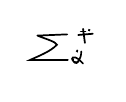
\begin{tikzpicture}[x=.22pt,y=-.22pt,baseline={(0,0)}]
\path[use as bounding box] (0,0) rectangle (116,76);
\node[overlay,anchor=base west,inner sep=0,outer sep=0] at (0,0) {\phantom{$\Sigma_\alpha^+$}};
% path C023-G18-P01: joined head and Sigma body.
\draw[line width=.62pt,line cap=round] (16,13) -- (65,11) (16,13) .. controls (31,19) and (46,23) .. (48,28) .. controls (38,39) and (17,47) .. (4,53) -- (66,53);
% path C023-G18-P02: lower alpha's complete retraced loop and arm.
\draw[line width=.60pt,line cap=round] (88,39) .. controls (88,51) and (82,61) .. (76,56) .. controls (68,48) and (77,46) .. (84,52) -- (91,59) (74,49) .. controls (73,57) and (80,61) .. (83,56);
% path C023-G18-P03: point above-left of alpha, separate from its body.
\fill (79,39) -- (81,36) -- (83,37) -- (82,41) -- cycle;
% path C023-G18-P04: plus's vertical and main horizontal.
\draw[line width=.63pt,line cap=round] (91,2) -- (94,25) (83,12) -- (107,10);
% path C023-G18-P05: short additional upper cross-run on plus.
\draw[line width=.56pt,line cap=round] (87,6) -- (95,6);
% path C023-G18-P06: tiny point above-right of plus, once.
\fill (100,2) -- (103,3) -- (102,6) -- (99,5) -- cycle;
\end{tikzpicture}}};
% END GROUP C023-G18
\node[anchor=base west,inner sep=0,outer sep=0] at (1481,1962) {$(\alpha\in K)$};
\node[anchor=base west,inner sep=0,outer sep=0] at (326,2128) {et de};
\node[anchor=base west,inner sep=0,outer sep=0] at (689,2100) {$V=X\setminus$};
% BEGIN GROUP C023-G19
% Nested origin (1045,2004), rectangle (0,0)--(94,105), baseline (0,0).
% Owns S11: the distinct roof, separate short head, body, plus and alpha.
% Roof is firm; the lower short head's head-versus-independent-run role remains local and unresolved.
\node[anchor=base west,inner sep=0,outer sep=0] at (1045,2004) {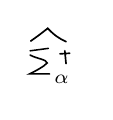
\begin{tikzpicture}[x=.22pt,y=-.22pt,baseline={(0,0)}]
\path[use as bounding box] (0,0) rectangle (94,105);
\node[overlay,anchor=base west,inner sep=0,outer sep=0] at (0,0) {\phantom{$\widehat\Sigma_\alpha^+$}};
% path C023-G19-P01: roof, separate from both the head and body.
\draw[line width=.61pt,line cap=round] (5,22) .. controls (15,15) and (23,9) .. (33,1) .. controls (43,12) and (52,18) .. (63,23);
% path C023-G19-P02: short separate head below the roof.
\draw[line width=.55pt,line cap=round] (4,38) -- (34,34);
% path C023-G19-P03: Sigma body and lower arm.
\draw[line width=.58pt,line cap=round] (4,45) .. controls (15,51) and (31,52) .. (32,58) .. controls (25,65) and (15,70) .. (3,76) -- (36,76);
% path C023-G19-P04: raised plus.
\draw[line width=.60pt,line cap=round] (53,43) -- (69,42) (61,38) -- (63,59);
\node[anchor=base west,inner sep=0,outer sep=0] at (44,91) {$\scriptstyle\alpha$};
\end{tikzpicture}};
% END GROUP C023-G19
% label C023-G15-L02: terminal full stop of the statement, once.
\node[anchor=base west,inner sep=0,outer sep=0] at (1183,2087) {.};
\end{tikzpicture}}
% END GROUP C023-G15

% BEGIN GROUP C023-G20
% Full-scan origin (435,2148); rectangle (0,0)--(340,89); baseline (0,58).
% Owns the complete Immédiat/Immèdiat/Immediat word and its lower-left faint trace M05.
% par remains outside. Accent candidates concern this word alone.
\begin{tikzpicture}[x=.18pt,y=-.18pt,baseline={(0,58)}]
\path[use as bounding box] (0,0) rectangle (340,89);
\node[anchor=base west,inner sep=0,outer sep=0] at (0,58) {\unsure{Immédiat|Immèdiat|Immediat}};
\node[anchor=base west,inner sep=0,outer sep=0] at (10,40) {\unsure{\begin{tikzpicture}[x=.18pt,y=-.18pt,baseline={(0,0)}]
\path[use as bounding box] (0,0) rectangle (10,16);
% path C023-G20-P01: short faint hook, separate from the first capital's main stroke.
\draw[black!35,line width=.24pt,line cap=round] (2,2) .. controls (5,6) and (7,9) .. (6,13);
\end{tikzpicture}}};
\end{tikzpicture}
% END GROUP C023-G20
 par \unsure{récurrence|rècurrence|recurrence} sur $\operatorname{card} K\geq 0$.
% archive sheet number: 22
